% !TEX root = tesis.tex

\chapter{Telescopio centellador de Rayos Cósmicos}
\chaptermark{Telescopio centellador}
\label{chap:dos}

Actualmente los telescopios de neutrones solares solo permiten estudiar el espectro de energía de manera parcial, es decir, con resolución limitada. Dado que los neutrones tienen masa, sus velocidades sufren dispersión dependiendo de su energía, lo cual complica establecer el perfil temporal de emisión. Aunado a esto, la baja estadística de conteo producto de la eficiencia de los telescopios y su limitada resolución angular; limitan las posibilidades de los TNS para esclarecer los mecanismos de aceleración de partículas.

Un diseño mejorado de Telescopio de neutrones fue propuesto en \cite{sako03}. En este diseño se utilizan barras de centelleo de dimensiones \SI[product-units=power]{5x10x300}{\cm}, alineadas de tal forma que permiten trazar las trayectorias de los neutrones incidentes además de medir su energía depositada. El Telescopio centellador de Rayos cósmicos (\emph{SciCRT} por sus siglas en inglés) es un nuevo experimento de rayos cósmicos basado en este principio.

El \emph{SciCRT} utiliza como trazador activo el detector \emph{SciBar}, diseñado originalmente para el experimento \emph{long-baseline K2K} \cite{knitta04} y posteriormente en el experimento \emph{SciBooNE} del \emph{Fermilab} (Laboratorio Nacional Fermi) \cite{hiraide06}. En el año \num{2013} el \emph{SciBar} fue trasladado a la cima del volcán Sierra Negra, Puebla a \SI{4600}{\metre} sobre el nivel del mar, con el objetivo de observar neutrones solares. La localidad de Sierra Negra es ideal para este experimento debido a la profundidad atmosférica (en línea vertical: \SI{575}{\gram\per\square\centi\metre}), su cercanía con el ecuador terrestre ($\ang{19.0}\mathbf{N}$, $\ang{97.3}\mathbf{W}$) , además de la experiencia previa en la operación de otro telescopio de neutrones solares en el sitio y la infraestructura del lugar\footnote{En la actualidad el volcán Sierra Negra se ha convertido en un observatorio astrofísico de nivel mundial.}.

Un diagrama esquemático del detector se muestra en la figura \ref{fig:scibar-detector}. Las ventajas del \emph{SciCRT} sobre la generación previa de telescopios proviene de integrar las funciones de anti-coincidencia, blanco centellador y telescopio direccional en las barras centelleo del \emph{SciBar}. Esto permite tener \num{15} veces más volumen activo, mejor resolución en energía y un umbral de detección menor. Considerando todas estas características el \emph{SciCRT} tiene una eficiencia detección \num{10} veces mayor a la del TNS previamente en el mismo sitio \cite{ynagai14} (considerando neutrones de \SI{100}{\mega\electronvolt}).

\begin{figure}
        \centering
        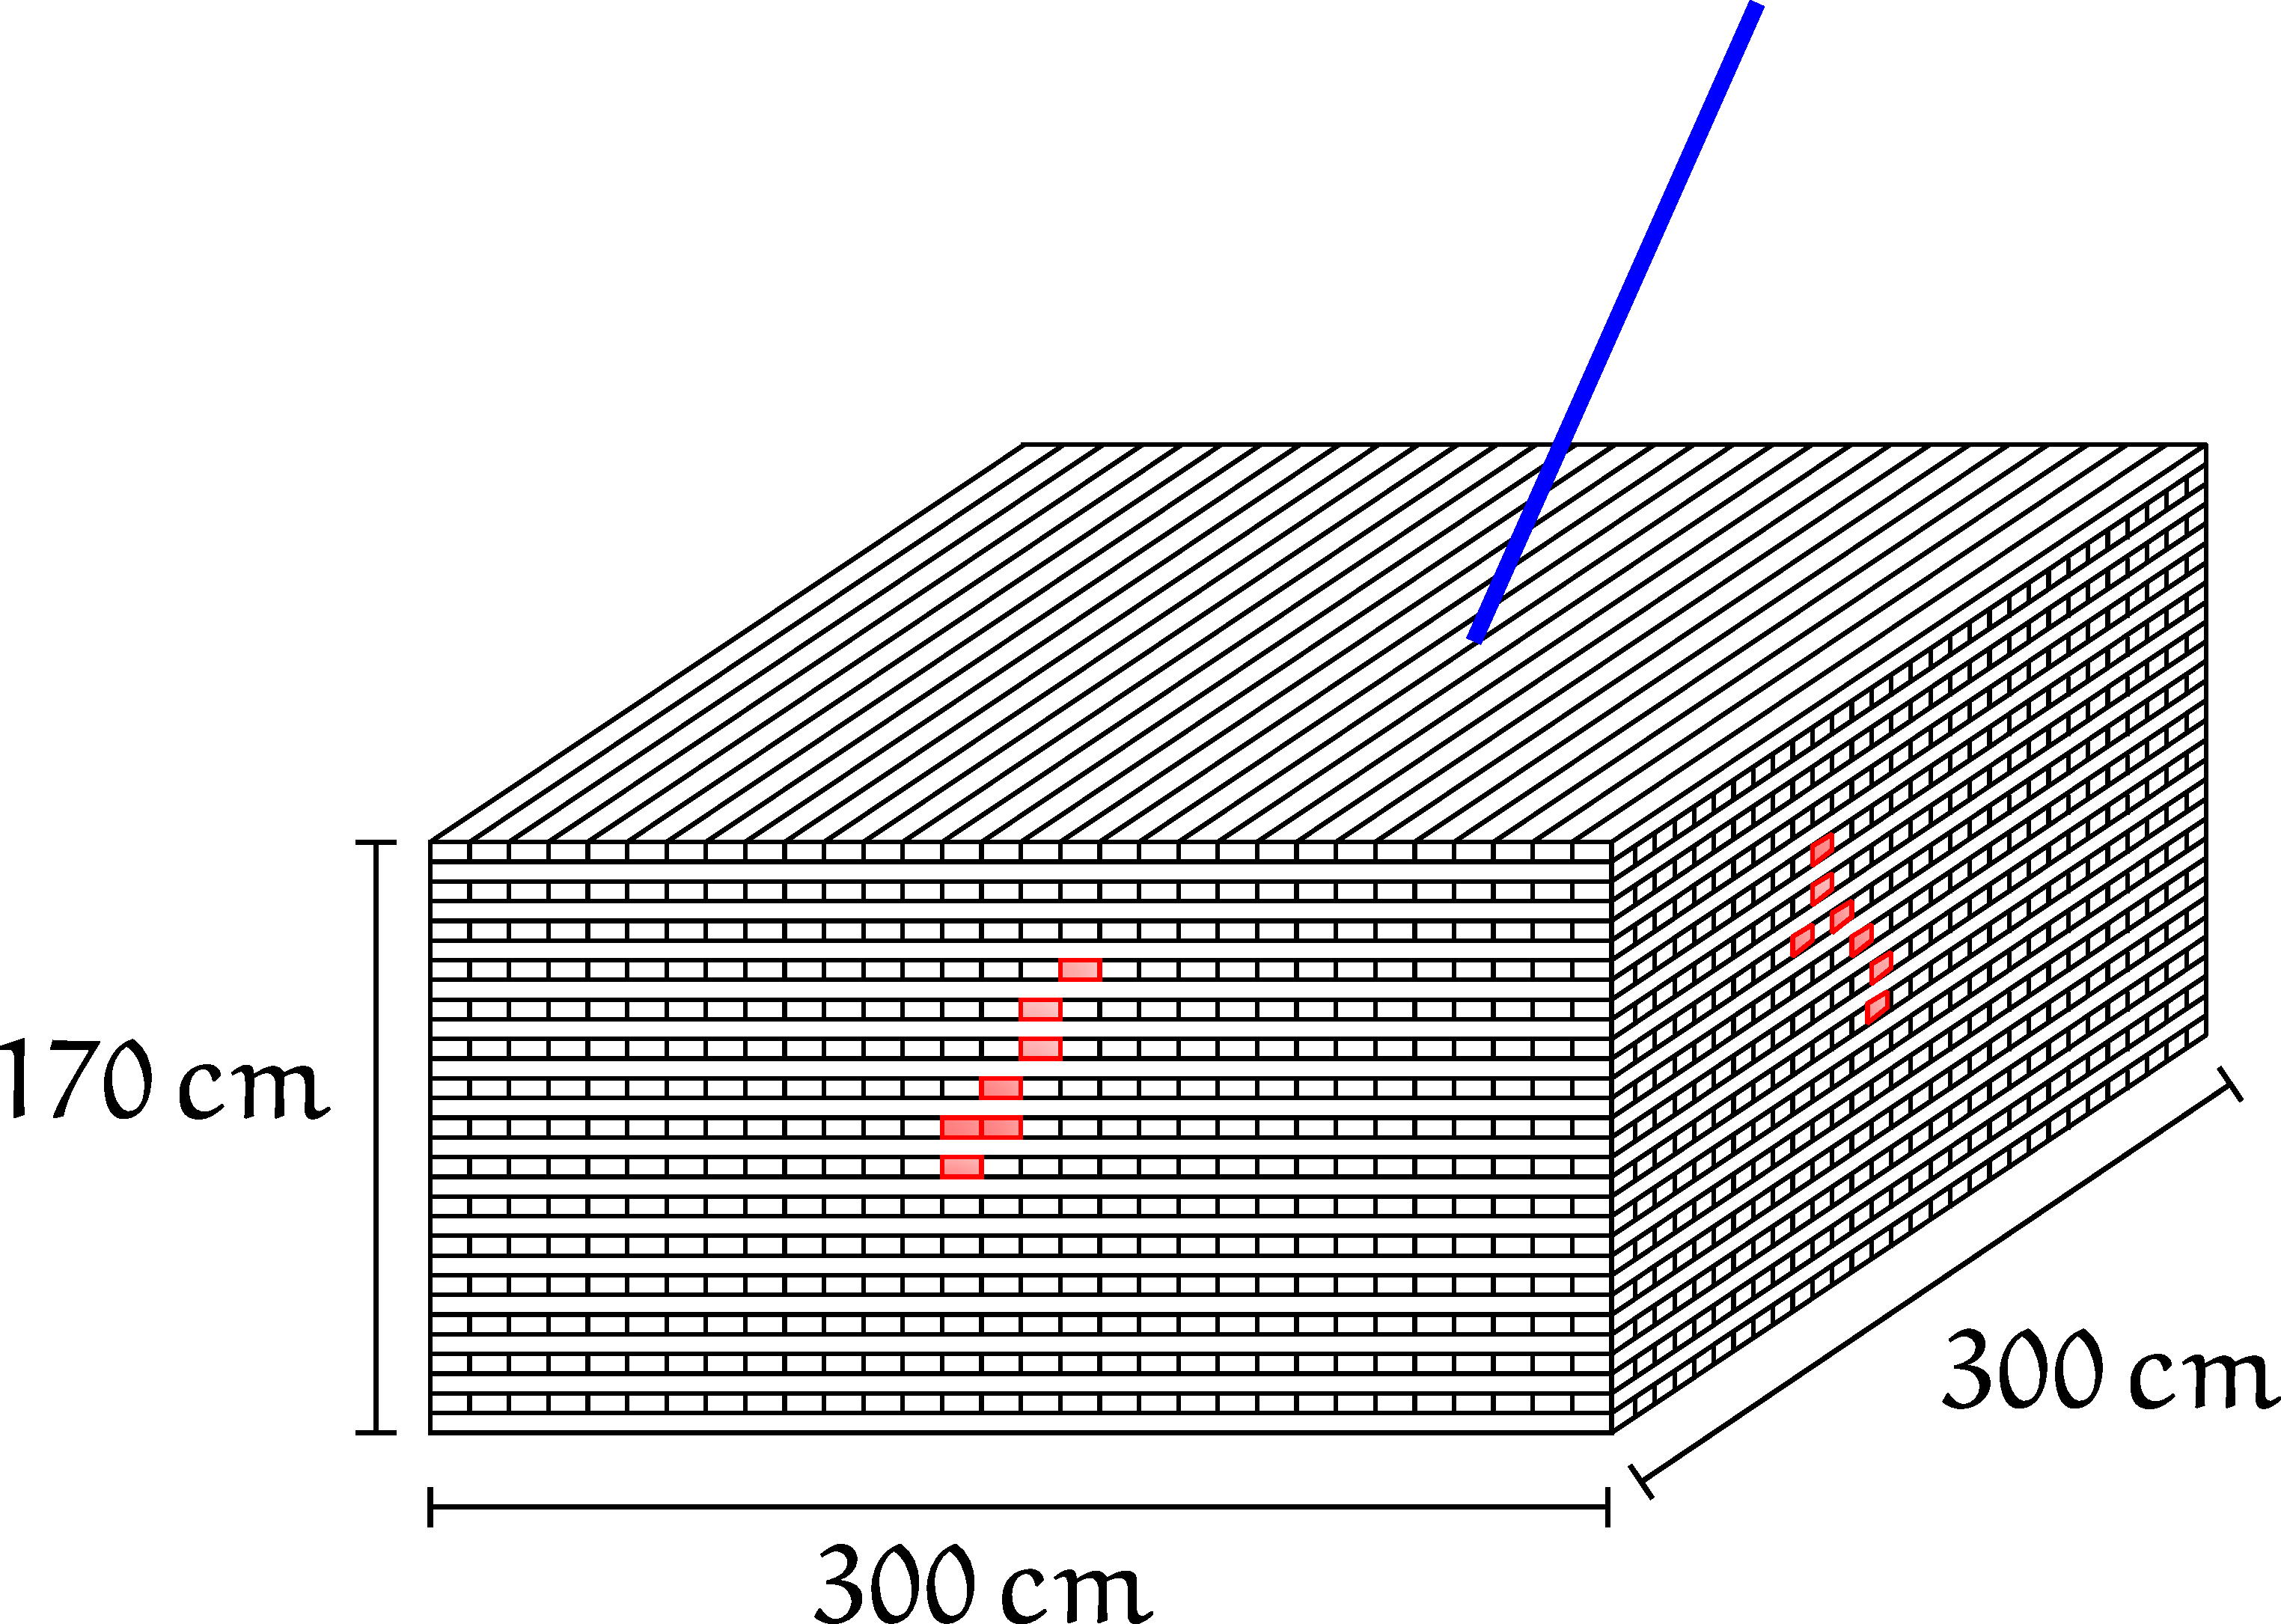
\includegraphics[width=0.7\textwidth]{scibar-diagram.pdf}
        \caption{Diagram esquemático del \emph{SciCRT}. El detector se compone de \num{14848} barras centelladoras y fibras \emph{WLS}. La lectura de las fibras se hace por medio \emph{MAPMT}s en grupos de \num{64} canales.}
        \label{fig:scibar-detector}
\end{figure}

Por otro lado, dado que el \emph{SciCRT} registra la energía depositada a lo largo la trayectoria de las partículas dentro del detector, podemos aplicar esquemas novedosos de identificación de partículas; lo cual a su vez mejora la sensibilidad a las partículas solares \cite{garcia20}. Este tipo de análisis \emph{offline} en conjunción con el uso de las barras de centelleo en modo anti-coincidencia mejora el rechazo a partículas de fondo (principalmente $\mu^{\pm}$ y rayos $\gamma$) incrementando la razón señal a ruido.

\section{Descripción del detector}

El \emph{SciCRT} está compuesto de \num{14848} barras de centelleo, alineadas en planos horizontales $X-Y$, perpendiculares entre si. Los planos están constituidos de \num{116} barras en la dirección $X$ y \num{118} en la dirección $Y$. En total hay \num{128} capas de barras de centelleo apiladas verticalmente, agrupada en estructuras de \num{16} capas llamadas \emph{Super block} (\emph{SB}). Cada \emph{SB} está sostenido firmemente por una estructura de acero, la cual mantiene la integridad mecánica de las barras. No obstante, la estructura introduce un hueco de aire entra cada capa de \SI{82}{\mm}, lo cual entre otras cosas afecta la respuesta angular del telescopio; por lo que es necesario incluir esta característica en las simulaciones del detector. El volumen total del barras en el detector es de \SI[product-units=power]{300x300x170}{\cubic\cm}.

Las barras de centelleo fueron fabricadas en el Fermilab y tienen características similares a las del experimento \emph{MINOS} \cite{knitta04}. Están hechas de poliestireno, dopado con \SI{1}{\percent} \emph{PPO} and \SI{0.03}{\percent} \emph{POPOP} (ambos utilizados como \emph{cambiadores} de longitud de onda). Las dimensiones de las barras son \SI[product-units=power]{2.5x1.3x300}{\cubic\cm} y en el centro tienen un orificio cilíndrico de \SI{1.8}{\mm} donde se insertan fibras \emph{WLS} (\emph{wavelength shifting}). Los centelladores tienen una cubierta de \ce{TiO2} (\SI{0.25}{\mm} de espesor) para aislarlos ópticamente entre si y mejorar la recolección de fotones. Un diagrama de las barras se observa en el panel izquierdo de la figura \ref{fig:scibar-optics}.

Las fibras \emph{WLS} están acopladas por un lado a un tubo fotomultiplicador multi-ánodo (\emph{MAPMT}) y por el otro extremo están pintadas de blanco para mejorar la eficiencia de recolección. Las fibras son del tipo Y11(200)MS desarrollado por la empresa \emph{Kuraray}. El fotomultiplicador es de \num{64} canales, modelo H8804, fabricado por \emph{Hamamatsu Photonics}.

El espectro de emisión de los plásticos centelladores se puede observar en el panel derecha de la figura \ref{fig:scibar-optics}, con una respuesta máxima a \SI{420}{\nano\metre}. Como se observa en la figura, el espectro de absorción de la fibra \emph{WLS} está diseñado para cubrir de forma adecuada el espectro del plástico. La emisión de la fibra tiene un máximo a \SI{470}{\nano\metre}. La máxima eficiencia cuántica del \emph{MAPMT} es de \num{0.25} a \SI{420}{\nano\metre}, pero disminuye a \num{0.12} al considerar el respuesta espectral del \emph{MAPMT}.

\begin{figure}
        \centering
        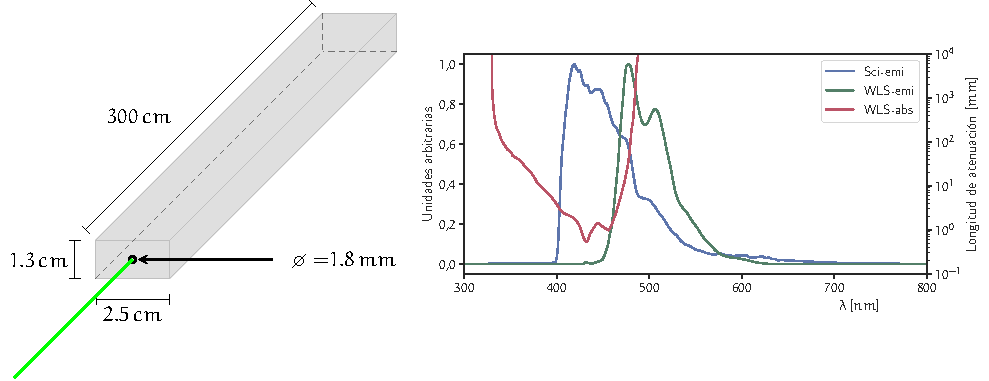
\includegraphics[width=\textwidth]{scibar.pdf}
        \caption{Diagrama esquemático de una barra centelladora con la fibra \emph{WLS} instalada (panel izquierdo). Espectros de absorción y emisión de la fibra \emph{WLS} y la barra de centelleo. Los datos de los espectros fueron obtenidos de \cite{kikawa14} y \cite{dietz16}.}
        \label{fig:scibar-optics}
\end{figure}

La electrónica para la adquisición de datos del telescopio fue desarrollada para el experimento K2K y esta integrada por circuitos de procesamiento analógico, de señal mixta y digitales; integrados a través de tecnología de circuitos integrados de alta escala \cite{myoshi04}. El procesamiento de la señales empieza con la conversión de la señal óptica en eléctrica por parte del \emph{MAPMT}, para posteriormente ser amplificada, formada y multiplexada en la electrónica de \emph{Front End}. Este acondicionamiento se lleva a cabo en el dominio analógico y de señal mixta. Después de este proceso, las señales se transfieren a la electrónica de \emph{Back End} mediante un bus diferencial. En las unidades que integran la electrónica de BE las señales son convertidas a digital y transferidas finalmente al servidor de adquisición de datos mediante la interface VME. Para poder seleccionar los eventos a guardar, las unidades FE mandan una señal de \emph{hit} a las tarjetas de disparo (TRGB), las cuales son unidades de procesamiento digital programable, que seleccionan los eventos con base a una condición de disparo. Una discusión más profunda sobre el funcionamiento de la electrónica se encuentra en el capitulo \ref{chap:tres}, en donde además se listan requerimientos y características de la nueva electrónica a desarrollar.

Bajo condiciones normales, el telescopio registra dos conjuntos de datos diferentes. Muones de alta energía (arriba de \SI{450}{\mega\electronvolt}) son detectados cuando producen coincidencia en las capas superiores e inferiores del detector. El umbral para la detección de partículas en las capas dedicadas es de \SI{0.3}{MIP} (\SI{\approx 0.5}{\mega\electronvolt}). El otro conjunto de datos del telescopio registra partículas neutras (aproximadamente \SI{70}{\percent} de los datos son de neutrones atmosféricos). El disparo para este tipo de eventos está definido cuando no hay ninguna señal en la capa de muones (anti-coincidencia) y además se registra una traza en uno de los \emph{SB} con al menos \SI{14}{\mega\electronvolt} de energía depositada. Las ganancias de los \emph{MAPMT} y umbrales para las capas de neutrones y muones se determinaron mediante simulaciones MC y se calibraron en Abril de \num{2014} \cite{ysasai14}.

\section{Caracterización del sistema óptico: barra de centlleo y fibra WLS}

Para lograr alcanzar los objetivos planteados, el siguiente paso de mi investigación fue la caracterización de los elementos ópticos y opto-electrónicos que integran al \emph{SciCRT}. Esto tuvo como objeto poder crear un modelo del proceso de generación de la señal de detección (simulación MC) y la posterior calibración de la electrónica usando dicho modelo.

Como ya mencioné anteriormente, las barras de centelleo del detector fueron fabricadas en Fermilab y han sido utilizados en diversos experimentos; por la misma razón sus propiedades ópticas y mecánicas han sido investigadas ampliamente. Como referencia me base unicamente en los datos del fabricante \cite{beznosko}.

El fluor usado en los plásticos del \emph{SciCRT} (\emph{POPOP} y \emph{PPO}) emite en el espectro visible desde aproximadamente \SI{400}{\nano\metre} hasta \SI{580}{\nano\metre}, con un máximo en la emisión de \SI{420}{\nano\metre} \cite{kikawa14}. El espectro de emisión de la barra se puede observar en color azul en el panel derecho de la figura \ref{fig:scibar-optics}. Por otro lado, la figura \ref{fig:sim-optics} muestra el resultado de simular \num{1e6} muones interaccionando una barra centelladora descrita usando \emph{Geant4} \cite{geant403,geant406} (distribución en color azul). Las características del modelo de la barra descrito se resumen en la tabla \ref{table:optics}.

\begin{figure}
        \centering
        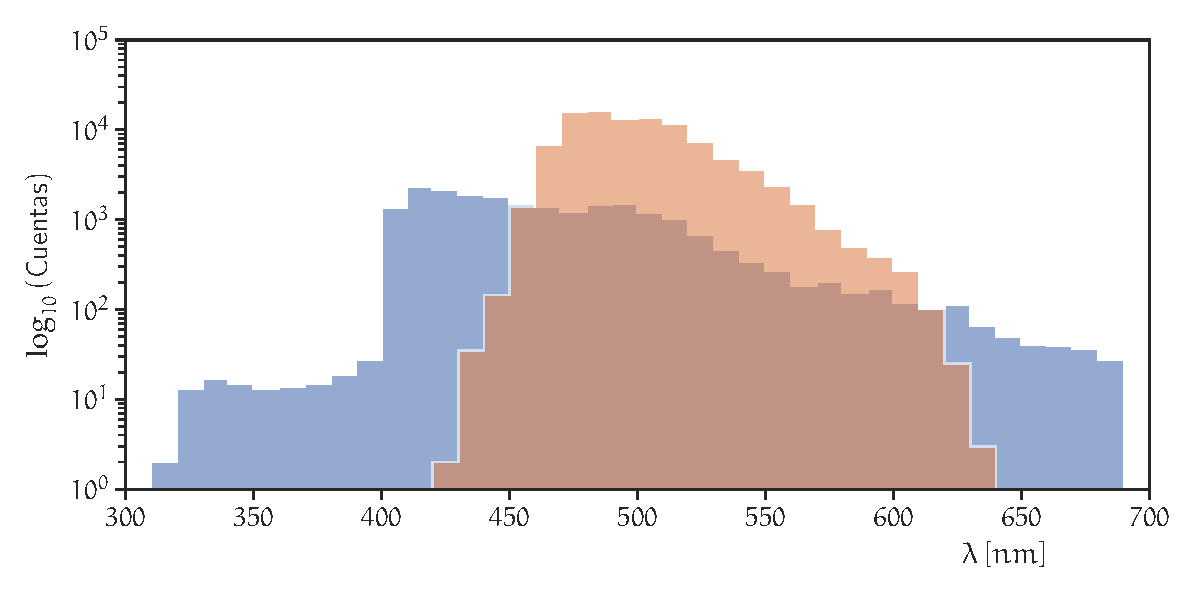
\includegraphics[width=\textwidth]{sim-optics-spect.pdf}
        \caption{Simulación MC del proceso de emisión-absorción de fotones entre la barra y la fibra \emph{WLS}.}
        \label{fig:sim-optics}
\end{figure}

Al ser excitadas las moléculas de la barra, los fotones son emitidos de forma isotrópica en el volumen del plástico. Para mejorar la recolección por parte de la fibra WLS y para aislar ópticamente las barras entre si, cada centellador cuenta con un recubrimiento de \ce{TiO2}. El espesor del recubrimiento impone una cota minima en la energía del primario que puede entrar en la barra y producir una señal detectable. De acuerdo con \cite{gros18}, resultados de una simulación MC sugieren que con un espesor similar al de las barras del \emph{SciCRT}; el flujo de protones, electrones y fotones con $E_{k}<\SI{10}{\mega\electronvolt}$ es atenuado considerablemente. En el caso de nuestro detector este efecto es despreciable ya que el umbral de detección de primarios (para todas las especies) se encuentra cercano a \SI{100}{\mega\electronvolt}.

En nuestra simulación de la barra un aspecto de vital importancia para la generación de las señales ópticas es el acoplamiento óptico que existe entre la superficie de la barra y el revestimiento. Tomando en consideración \cite{dietz16,gros18}, fijé la reflectividad del recubrimiento en \SI{90}{\percent} en el rango de \SI{300}{\nano\metre} a \SI{800}{\nano\metre}, considerando además una componente difusa y especular. Dicho de otra forma, esta caracterización garantiza que la simulación trata la reflexión de los fotones en el recubrimiento de manera geométrica, engrosando en el espectro de los fotones de acuerdo a un cierto parámetro de rugosidad; lo cual simula las imperfecciones en ambas superficies.

Una fracción de los fotones que llegan a entrar en la fibra WLS son absorbidos y reemitidos a una mayor longitud de onda que la inicial\footnote{Por efecto de la conservación de la energía el fotón reemitido nunca puede tener una longitud menor a la longitud inicial.}. La emisión de los fotones por la fibra tiene las características de un decaimiento exponencial con $\lambda_{WLS}=\SI{12.0}{\nano\second}$ y es isotrópica. Debido a que la fibra tiene dos recubrimientos (metacrilato y metacrilato fluorado) para que se lleve a cabo la reflexión total interna se requiere que los fotones sean emitidos con ángulos menores a \SI{26.9}{\degree} con respecto al eje de la fibra \cite{kikawa14}.

\begin{table}
\caption{Características ópticas y mecánicas.}
\label{table:optics}

\begin{tabular}{lr}

\multicolumn{2}{c}{}\\
\cmidrule(r){1-2}
\addlinespace[5pt]
\textbf{(a) Barra centelladora}\\
\addlinespace[5pt]
\cmidrule(r){1-2}
Material base & poliestireno\\
Fluor & \emph{PPO} y \emph{POPOP}\\
Densidad (\si{\gram\per\cubic\cm}) & \num{1.08}\\
Pico de emisión (\si{\nm}) & \num{420}\\
Constante de decaimiento (\si{\ns}) & \num{3.6}\\
Constante de Birks (\si{\cm\per\mega\electronvolt}) & \num{0.0208}\\
Producción de luz (\si{fotones\per\mega\electronvolt}) & \num{8000}\\
Dimensiones (\si{\cubic\cm}) & \num[product-units=power]{2.5x1.3x300}\\
\addlinespace[10pt]
\textbf{(b) Fibra WLS Y11(200)}\\
\addlinespace[5pt]
\cmidrule(r){1-2}
Densidad (\si{\gram\per\cubic\cm}) & \num{1.05}\\
Pico de emisión (\si{\nm}) & \num{470}\\
Longitud de absorción & ver figura \ref{fig:scibar-optics}\\
Índice de refracción (núcleo) & \num{1.60}\\
Índice de refracción (revestimiento 1) & \num{1.49}\\
Índice de refracción (revestimiento 2) & \num{1.42}\\
Tiempo de decaimiento (\si{\ns}) & \num{12.0}\\
Reflectancia de la pintura & 0.54\\
\addlinespace[10pt]
\textbf{(c) MAPMT H8804}\\
\addlinespace[5pt]
\cmidrule(r){1-2}
Longitud de onda de respuesta máxima(\si{\nm}) & \num{420}\\
QE máxima (\si{\percent})  & \num{25}\\
Ganancia a \SI{-950}{\volt} & \num{5.9e6}\\
Tiempo de levantamiento (\si{\ns}) & \num{1.0}\\
\addlinespace[5pt]
\bottomrule

\end{tabular}
\end{table}

Los parámetros usados en la simulación de la fibra en \emph{Geant4} se muestran en la tabla \ref{table:optics}. Es importante hacer notar que todos los parámetros ópticos utilizados fueron definidos en el rango de \SI{300}{\nano\metre} a \SI{800}{\nano\metre}, lo cual requirió en algunos casos extrapolar cuidadosamente los datos proporcionados por el fabricante. Relacionado a este punto, ese necesario evitar introducir discontinuidades en los espectros definidos, ya que dicha situación conlleva a la creación de acoplamientos ópticos artificiales y por lo tanto a la atenuación de la señal óptica. En la figura \ref{fig:sim-optics}, la distribución en color naranja muestra los fotones reemitidos en la simulación, los cuales constituyen una prueba de la consistencia de la simulación.

Dentro de los parámetros de la simulación, la longitud de atenuación óptica de la fibra WLS requirió una calibración especial. La figura \ref{fig:atlength} muestra los resultados de este procedimiento. Como primer paso, la línea naranja es el resultado de la simulación previo a la calibración. La simulación consistió en arrojar fotones usando el espectro de emisión de la barra, a diferentes posiciones fijas dentro de la fibra y de manera isótropica. En la simulación usé como parámetro de entrada la longitud de atenuación propuesta por el fabricante: $>\SI{3500}{\milli\metre}$, la cual se define en \emph{Geant4} como una propiedad del material (en este caso del núcleo de la fibra). Para cada posición la simulación registra el número de fotones que llegaron al extremo de la barra donde se encuentra el fotosensor. Luego entonces, los resultados en la figura \ref{fig:atlength} son el número de fotones (normalizado) $L(x)$ que alcanzan el \emph{MAPMT}en función de la distancia al mismo.

Los resultados de la simulación se pueden ajustar con la ecuación \ref{equ:fiber-att}, la cual representa la relación entre la distancia al fotomultiplicador y $L(x)$:

\begin{equation}
\label{equ:fiber-att}
L(x)=k\left(\exp\left(-\frac{x}{\lambda}\right) +R\exp\left(-\frac{2.0x_{tot}-x}{\lambda}\right)\right)
\end{equation}

de donde $k$ es la ganancia del sistema óptico, $\lambda$ es la longitud de atenuación, $R$ es la reflectancia de al final de la fibra WLS y $x_{tot}$ es la longitud total de la fibra (aproximadamente \SI{330}{\cm}, incluyendo la distancia del borde de la barra al fotomultiplicador). De manera general, el primer término de la ecuación representa la fracción de la luz que llega al \emph{MAPMT}directamente, mientras que el segundo término representa la fracción reflejada.

\begin{figure}
        \centering
        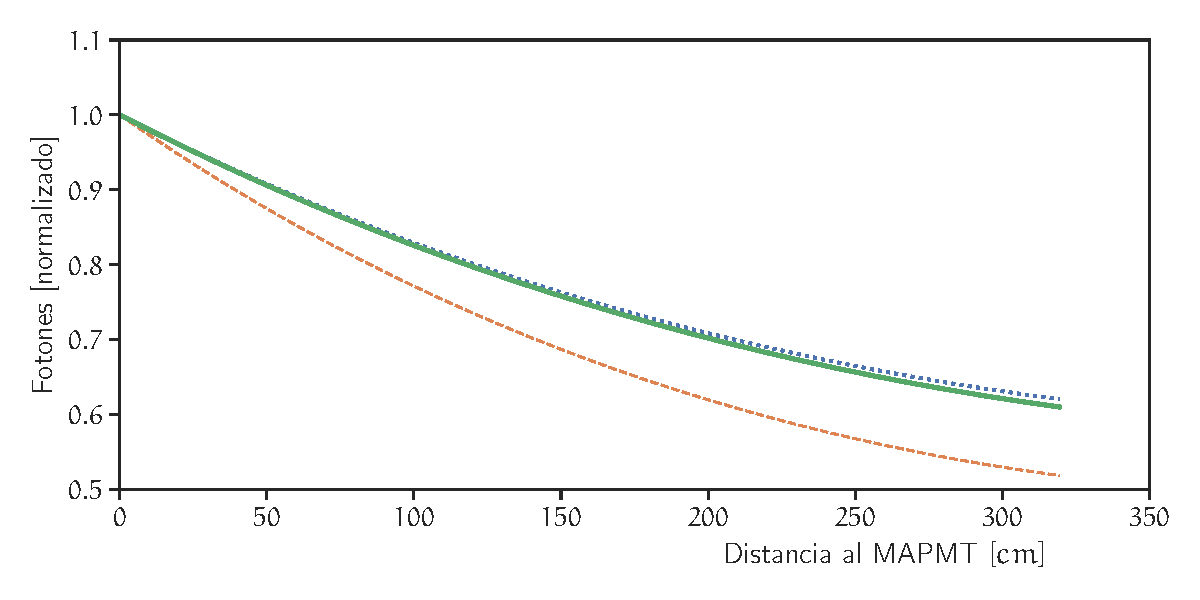
\includegraphics[width=\textwidth]{data_atlength.pdf}
        \caption{Atenuación de fotones en la fibra \emph{WLS}. La línea azul son datos del experimento. La línea naranja representa el resultado de la simulación MC usando la atenuación reportada por el fabricante. La línea verde es el ajuste de la simulación a partir del experimento.}
        \label{fig:atlength}
\end{figure}

El siguiente paso fue la obtención de la longitud de atenuación usando los datos del telescopio. Para determinar este parámetro, usé \num{\sim 4e6} eventos de muones, los cuales fueron registrados usando como disparo la coincidencia de las capas superiores e inferiores del detector (\emph{$4$-fold}). Utilicé muones para esta prueba debido a que son partículas de ionización mínima (\emph{MIP}) y su deposición de energía en una barra es prácticamente constante (aproximadamente \SI{1.8}{\mega\electronvolt}).

A partir de los datos registrados, construí distribuciones de la energía depositada en cada barra de uno de los lados del detector; mientras la traza en la otra cara del detector sirve para medir la distancia entre el punto de cruce de la partícula y el MAPMT. Las distribuciones de cada barra se clasifican en $14$ grupos diferentes (hay \num{14} MAPMTs en una de las caras del \emph{SciCRT}), lo cual hace posible medir el efecto de atenuación en la fibra midiendo la posición del pico de la distribución de energía depositada en cada barra, en función de la distancia. Utilizando esta clasificación es posible medir la distancia del punto de cruce con un incertidumbre de \SI{\pm 10}{\cm}. Una restricción extra que establecí en el análisis fue la de analizar solo eventos producidos por partículas que cruzan de forma vertical, lo cual tiene por objetivo evitar eventos con una larga deposición de energía. La figura \ref{fig:muon-selection} muestra de forma resumida el procedimiento de selección de eventos y clasificación descrito.

Por otro lado la figura \ref{fig:adc-distance} muestra las distribuciones de ADC de muones cruzando a dos distancias diferentes del \emph{MAPMT}. La distribución en azul claro corresponde a una distancia de \SI{280}{\cm}, mientras que la distribución en azul oscuro la obtuve a \SI{40}{\cm}. Usando un voltaje de alimentación para el \emph{MAPMT} de \SI{-900}{\volt}, cerca \SI{50}{\percent} de las barras (de un total de \num{896}) tiene estadística suficiente para realizar el análisis, lo cual quiere decir que las distribuciones obtenidas no son afectadas por la saturación del \emph{MAPMT} o falta de ganancia.

\begin{figure}
        \centering
        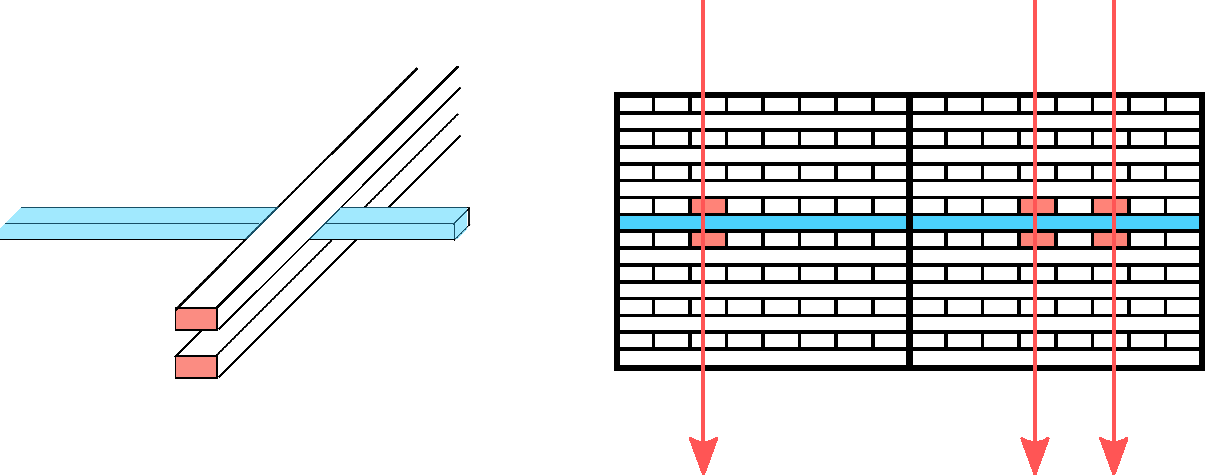
\includegraphics[width=\textwidth]{muon-attenuation.pdf}
        \caption{Diagrama esquemático de la selección de eventos de muones en los datos del \emph{SciCRT}.}
        \label{fig:muon-selection}
\end{figure}

\begin{figure}
        \centering
        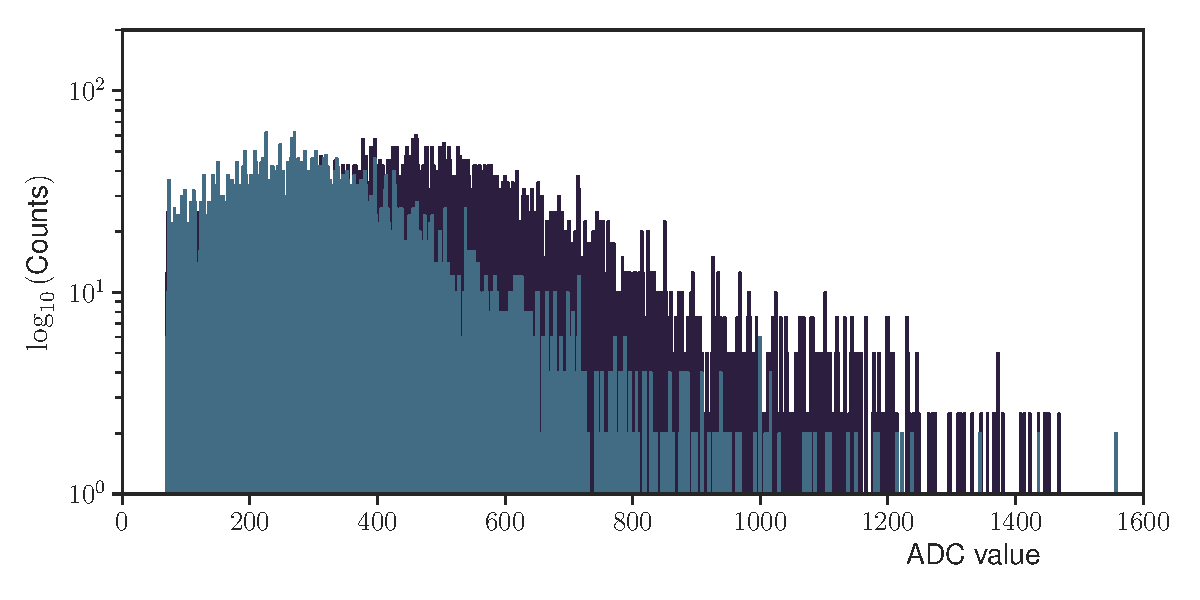
\includegraphics[width=\textwidth]{adc_attenuation.pdf}
        \caption{Distribuciones de ADC de muones que cruzan una barra de centelleo a diferentes distancias del fotomultiplicador.}
        \label{fig:adc-distance}
\end{figure}

Ya que los muones registrados en el análisis están el rango de energía de \num{0.5} a \SI{30}{\giga\electronvolt} y son considerados \emph{MIPs}, las distribuciones de intensidad luminosa registrada por los \emph{MAPMTs} pueden ser ajustadas utilizando distribuciones de Landau. A partir del valor máximo estimado en cada ajuste (\emph{MPV}) procedí a calcular el promedio ponderado para cada distancia. Posteriormente, ajusté la ecuación \ref{equ:fiber-att} y como resultado obtuve la gráfica azul mostrada en el figura \ref{fig:atlength}. Los parámetros obtenidos a partir del ajuste son: $\lambda=\SI{408(4)}{\cm}$ y $R=\num{0.541(30)}$, lo cual es consistente con un estudio previo \cite{itow13}.

No obstante, es evidente de la figura que el resultado experimental difiere del obtenido en la simulación, lo cual indica que es necesario ajustar los parámetros del código. La discrepancia entre ambos experimentos proviene de varios factores. El primero es que la longitud de atenuación provista por el fabricante es en realidad un \emph{longitud de atenuación de señal}, es decir, proviene de una medición realizada por el fabricante en donde interviene la geometría del experimento donde se midió y el acoplamiento óptico entre los diferentes elementos. Por otro lado en la simulación, la longitud de atenuación es una propiedad del material.

Con objeto de resolver esta discrepancia en \cite{dietz16} se propone utilizar el espectro de pérdidas de señal $\mu_{WLS}$, el cual se muestra en la figura \ref{fig:sim-optics} describe de mejor forma la atenuación en la fibra. Este espectro es provisto por el fabricante, sin embargo requiere un factor de corrección cuadrático:

\begin{equation}
\label{equ:quadcorr}
\mu_{corr}=a_{0}\cdot\mu_{WLS}+a{1}\cdot\mu^{2}_{WLS}
\end{equation}

en donde $\mu_{corr}$ es el espectro corregido y $\mu_{WLS}$ es el especificado por el fabricante. De esta forma podemos usar las constantes $a_{0}$ y $a_{1}$ para calibrar los resultados de la simulación con el experimento. Finalmente, la linea verde en la figure \ref{fig:atlength} muestra el resultado de la corrección de la simulación, con parámetros de ajuste: $\lambda=\SI{405(3)}{\cm}$ y $R=\num{0.498(20)}$. A partir de esto podemos concluir que la simulación y experimento concuerdan satisfactoriamente.

\section{Caracterización del sistema óptico: respuesta del fotomultiplicador}


\begin{figure}
        \centering
        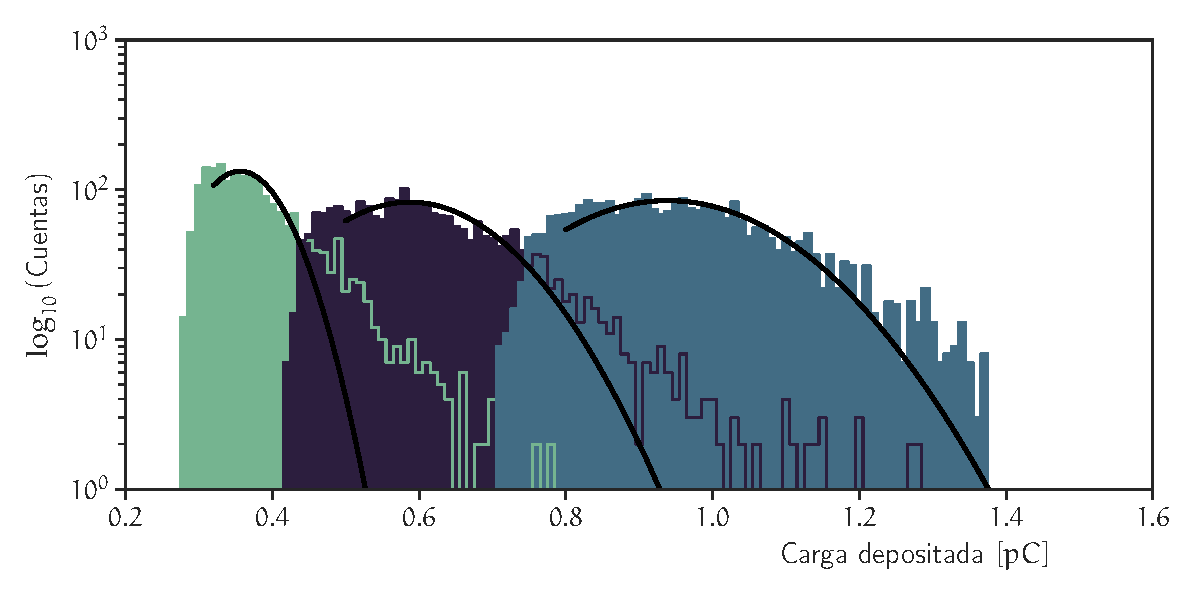
\includegraphics[width=\textwidth]{mapmt_charge.pdf}
        \caption{Distribuciones de carga de SPE para tres diferentes voltajes de operación. De izquierda a derecha los voltajes utilizados son: \SI{-800}{\volt},\SI{-850}{\volt} y \SI{-900}{\volt}.}
        \label{fig:mapmt_charge}
\end{figure}

\begin{equation}
\label{equ:sphe}
v(t)=\frac{QR}{\tau\Gamma(1+\alpha)}\left(\frac{t}{\tau}\right)^{\alpha}\mathrm{e}^{-t/\tau}
\end{equation}

\begin{figure}
        \centering
        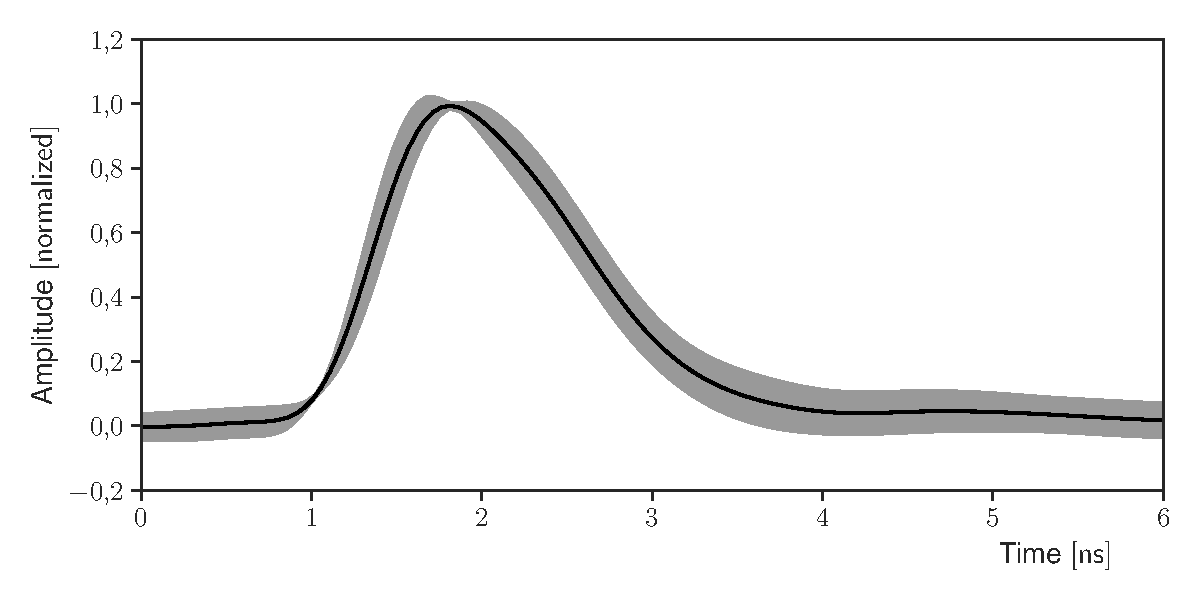
\includegraphics[width=\textwidth]{sphe-signal.pdf}
        \caption{Respuesta SPE promedio en función del tiempo (linea negra). El área sombreada muestra las fluctuaciones de $\pm\sigma$.}
        \label{fig:sphe}
\end{figure}

\section{Validación experimental de la simulación}



\begin{figure}
        \centering
        \includegraphics[width=\textwidth]{muons-experiment.pdf}
        \caption{Configuración del experimento en Sierra Negra. El sistema de coincidencias se forma por las tarjetas instaladas en las posiciones marcadas en verde.}
        \label{fig:muons-experiment}
\end{figure}


\begin{figure}
        \centering
        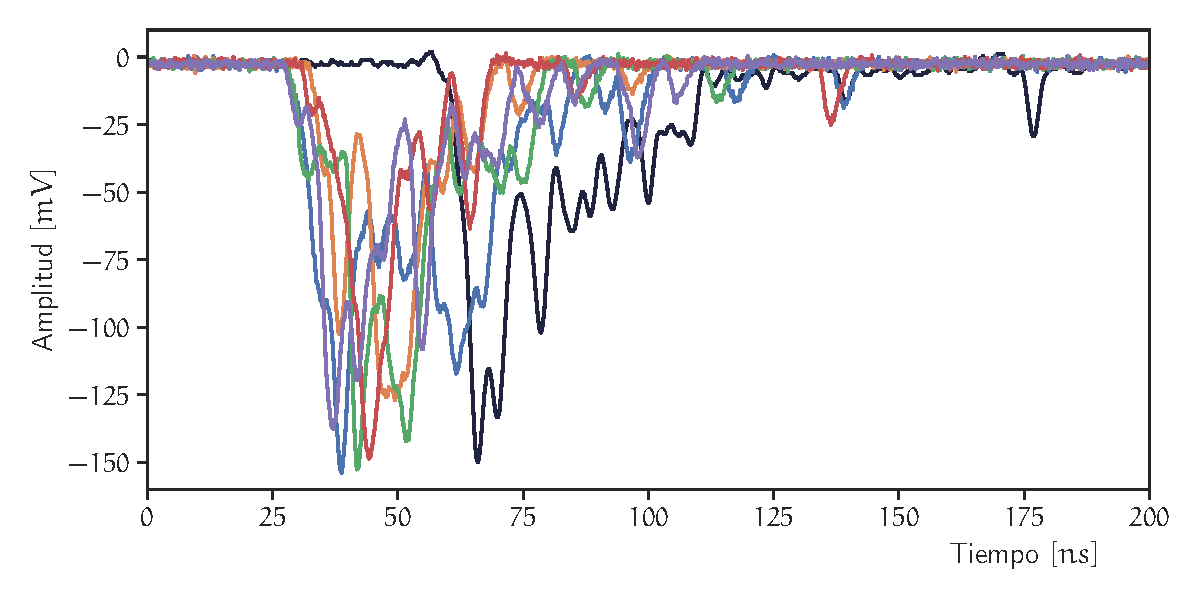
\includegraphics[width=\textwidth]{muon-pulse.pdf}
        \caption{Comparación entre señales generadas por la simulación MC (líneas de color) y el experimento realizado en Sierra Negra (línea oscura).}
        \label{fig:muon-pulse}
\end{figure}

\begin{figure}
        \centering
        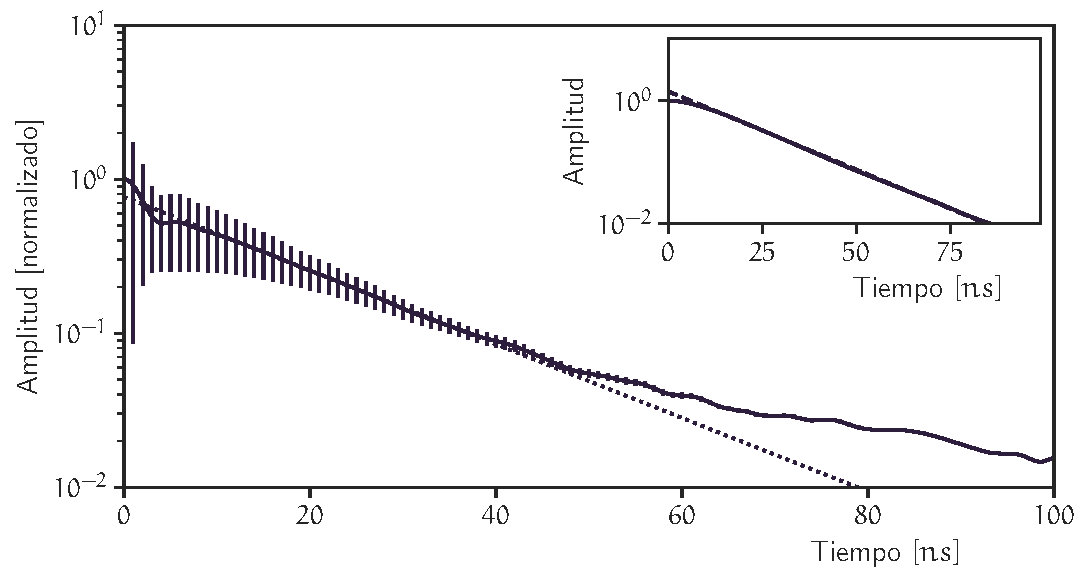
\includegraphics[width=\textwidth]{muons-tail-fit.pdf}
        \caption{Análisis del decaimiento exponencial de la fibra \emph{WLS}. El panel en la esquina superior derecha muestra los resultados de la simulación. Los datos experimentales se muestran en la parte central de la figura}
        \label{fig:muons-tail}
\end{figure}

\begin{equation}
\label{equ:nphe}
s(N_{phe})=\frac{1}{k_{sat}}\int_{0}^{N_{max}} s_{sim}(N_{sim})p(N_{phe}-N_{sim})\;\mathrm{d}N_{sim}
\end{equation}

\begin{figure}
        \centering
        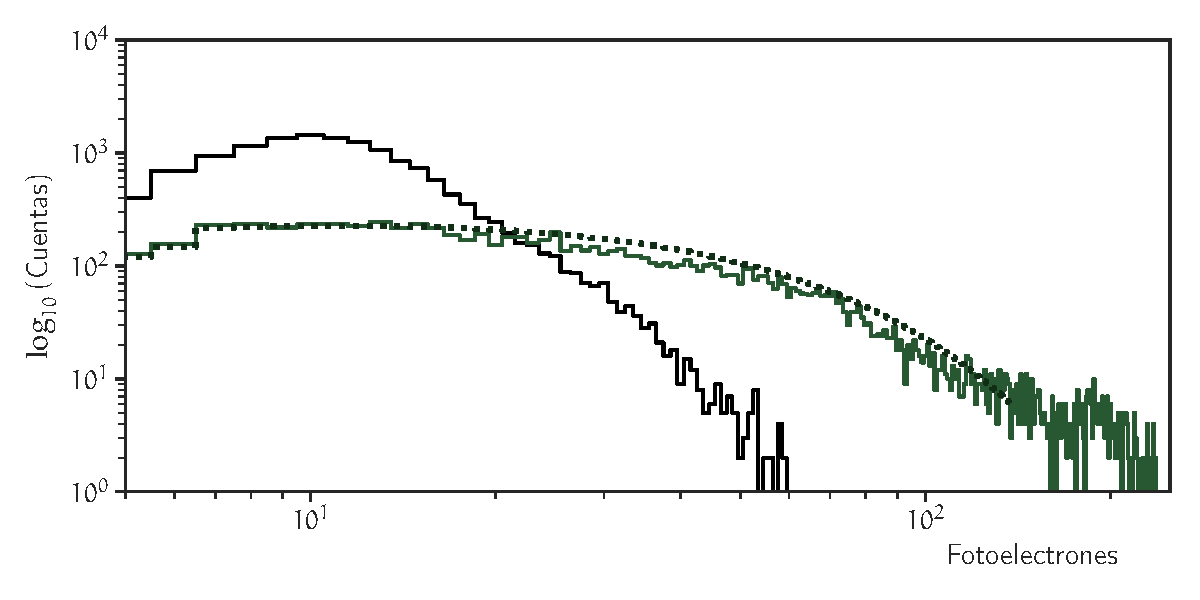
\includegraphics[width=\textwidth]{photons-number.pdf}
        \caption{Distribución de número de fotoelectrones detectados en el experimento y la simulación MC. Los resultados de la simulación se convolucionan con una función de resolución para ajustar con los datos experimentales.}
        \label{fig:photons-number}
\end{figure}
